\setchapterpreamble[u]{%
\dictum[René Descartes]{Vor eine Frage gestellt, die wir vollständig verstanden haben, müssen wir sie von jeder überflüssigen Darstellung abstrahieren, sie auf ihre einfachste Form reduzieren und sie in möglichst kleine Teile zerlegen, die wir dann aufzählen. \dots}}
\chapter{Analyse und Definition der Anforderungen } \index{Analyse und Definition der Anforderungen}\label{kap:analyse_und_definition}

Die ISO Standards 29002-31 und 22745-30 wurden vom Fachbereich als mögliche zu implementierende Standards genannt, um die Anforderungen einer Abfrageschnittstelle analog zu SQL-Möglichkeiten (Projektion, Selektion) zu gewährleisten.   

Mittels den Erkenntnissen der Analyse werden mögliche Use Cases erarbeitet. Wichtig ist auch zu evaluieren, welche Standards gegebenenfalls betrachtet und implementiert werden müssen, um die Anforderungen umzusetzen. 

\section{Analyse ISO 29002-31 - Exchange of characteristics data}

\todotext{Einen definierten Großteil in den Anhang packen. Hier nur ein Beispiel und das Ergebnis erklären}

\subsection{XML Datencontaineranalyse ISO 29002-31}\index{ISO 29002-31}
Die Unterkapitel beschreiben die einzelnen (XML) Datencontainer aus der ISO 29002-31. Der Ausgangspunkt ist der query\_context, welcher einige Metadaten zum eigentlichen query enthält. 

\begin{figure}[htbp]
	\centering
		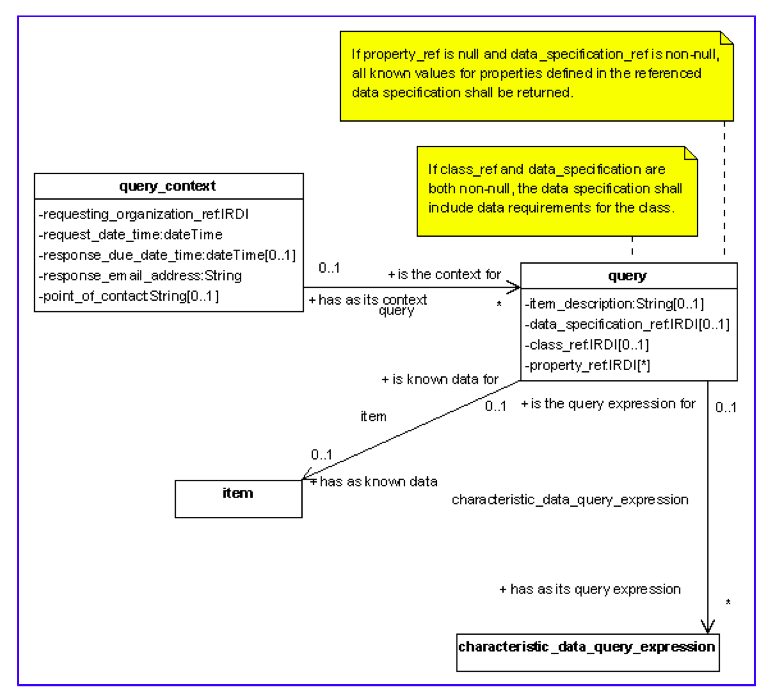
\includegraphics[width=0.99\textwidth]{images/query_main.png}
		\caption[UML-Diagramm Query Main]{UML-Diagramm Query Main\footnotemark}
	\label{fig:querymain}
\end{figure}
\footnotetext{Quelle: ISO 29002-31 Kapitel 5.2.1}

\subsubsection{query\_context}
Dies ist eine Art Container für eine Menge von Queries. Inhalt sind Informationen über den Anforderer der Daten zwecks persönlicher Kontaktaufnahme, wie z.B. die Anfragezeit, Informationen über die Organisation welche die Anfrage schickt sowie einen gewünschten Antwortzeitpunkt mit Antwort-Email Adresse. Siehe dazu \autoref{fig:querymain} und \citep[Kap. 5.2.2][]{iso29002-31}.  

Da die Vorgabe lautet, den Service auf Basis eines Web Services zu erstellen, entfällt die Benutzung des query\_context. Der Grund ist, dass der Kontext  implizit durch den Web Service respektive dem Server zur Verfügung gestellt wird. Beispielsweise wird die Anfragezeit zwar nicht explizit durch den Serviceaufrufer selbst übergeben, allerdings durch die Anfrage an den technischen Server wie z.B. Apache Tomcat Server mittels Logeintrag implizit ermittelt. Somit lassen sich diese Metadaten über Verbindungsprotokolle der Infrastruktur herausfinden.  
Siehe dazu auch \citep[Kap. 6][]{iso29002-31}, welche besagt: \\ \enquote{ISO/TS 29002 can be implemented: \\
a. with another envelope standard, such as EDI, or \\
b. by itself, using the query\_context to carry envelope information.}

\subsubsection{query}
Die Unterstützung aller Funktionalitäten des queries entspricht laut ISO 29002-31 der Conformance class 1: simple query \citep[Anhang 6][]{iso29002-31}. .
Dies ist der eigentliche Abfrage-Datensatz. Abgefragt werden kann mittels class IRDI\footnote{IRDI  - International registration data identifier}, data\_specification IRDI, eine Menge von property IRDI, Teiledaten (das sind Teile gefüllt mit Daten ihrer Eigenschaften die dem Klienten bereits bekannt sind) und einer item\_description. Das bedeutet, dass bereits bekannte Eigenschaften eines Teils übertragen werden können, um die Suche auf Teile mit diesen Werte-Eigenschaften einzuschränken.

Die data\_specification IRDI verweist auf eine Spezifikation aus ISO 22745-30, die besagt welche Properties für dieses Teil sinnvoll sind. Die angegebenen Property IRDIs sind dann eine Teilmenge aus den mittels data\_specification IRDI definierten erlaubten Eigenschaften. Für weitere Informationen zur ISO 22745-30 siehe \autoref{kap:identification_guide}. 

Ad hoc denkbar wären einfache Abfragen wie z.B.: \enquote{Gib mir alle Teile der Klasse xyz}. Mitgeliefert werden auch Teile von Subklassen. Weiterhin kann die Abfrage nach bestimmten Eigenschaften eingeschränkt werden. Eine weitere Möglichkeit ist es bereits bekannte Daten über ein Element zu übermitteln, mit dem Zwecke hierüber die IRDI zu erfahren oder weitere Eigenschafts-Daten zu erhalten. Siehe Beispielqueries simple queries in \autoref{kap:query_beispiele}. 

\subsubsection{characteristic\_data\_query\_expression (parametric\_query)}
Das entspricht laut ISO 29002-31 Anhang 6 der Conformance class 2: parametric query.

\begin{figure}[htbp]
	\centering
		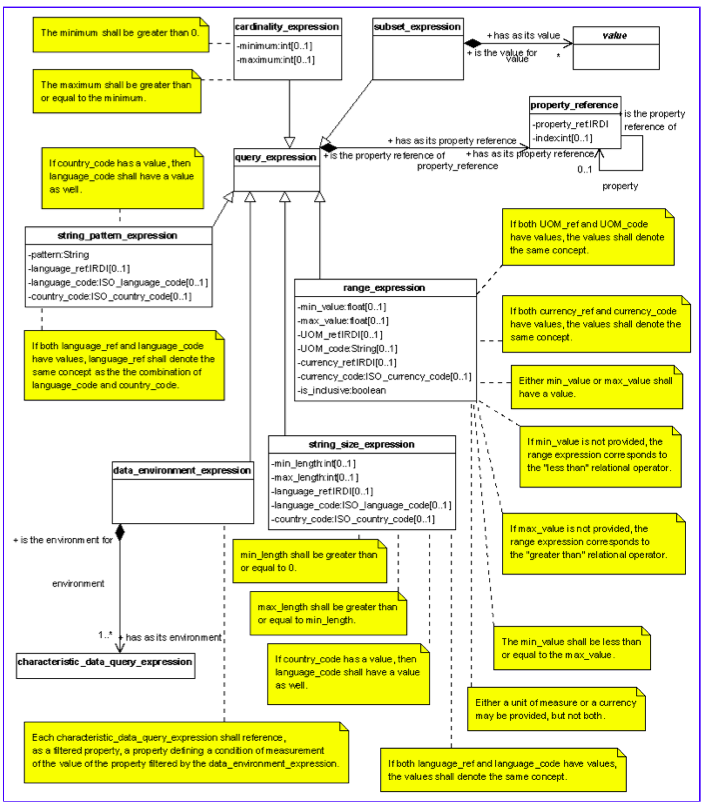
\includegraphics[width=0.99\textwidth]{images/query_expression.png}
		\caption[UML-Diagramm Query Expression]{UML-Diagramm Query Expression\footnotemark}
	\label{fig:querymain}
\end{figure}
\footnotetext{Quelle: ISO 29002-31 Kapitel 5.3.1}

Eine characteristic\_data\_query\_expression kann verschieden expressions vom Typ query\_expression beinhalten. Von jedem Typ jeweils nur maximal eine. 
Z.B.
\begin{itemize}
\item string\_size\_expression
\item string\_pattern\_expression
\item range\_expression
\item data\_environment\_expression
\item cardinality\_expression
\item subset\_expression
\end{itemize}
darüberhinaus noch folgende Attribute

\begin{itemize}
\item property\_reference - die property auf den die query\_expression bezogen ist
\end{itemize}
Solch eine Expression ermöglicht das Filtern, gleichsam ein Einschränken bestimmter Properties und Werte. 

\subsubsection{Query Beispiele}\label{kap:query_beispiele}

Nachfolgend seien einige Query-Beispielszenarien aufgestellt, die sich aus der Analyse der Standards ergeben.

Eine Schraube hat die folgenden möglichen Eigenschaften: 

\begin{description}
\item[Klassen-Identifier] 1234-abcd\# ab-cdefgh\# 1 (IRDI)
\item[Typ] M6 (Property IRDI: 1234-abcd\# ab-bbbbbb\# 1)
\item[Länge] 80mm (Property IRDI: 1234-abcd\# ab-cccccc\# 1)
\end{description}

\paragraph{Simple Query}\index{Query!Simple Query}

Ein simpler query ermöglicht folgende Abfrage: \enquote{Gib mir alle Teile zum Konzept Kreuzschraube mit dem Identifier (IRDI) 1234-abcd\#ab-cdefgh\#1}. Das Ergebnis ist ein Teil, mit allen Attributen wie oben angegeben. 

Ein anderer Query könnte lauten: \enquote{Gib mir die Properties 1234-abcd\#ab-cccccc\#1 und 1234-abcd\#bbbbbb\# 1 des Items der Klasse 1234-abcd\#ab-cdefgh\#1}. Das Ergebnis wäre das Teil mit Typ: M6 und der Länge: 80mm.

Es könnte auch mit Hilfe von vorhandenen Daten gesucht werden, z.B.:  \enquote{Hier ist ein Teil mit der Property Typ: M6 (Property IRDI: 1234-abcd\# ab-bbbbbb\# 1), gib mir bitte dazu die Properties 1234-abcd\#ab-cccccc\#1 und 1234-abcd\# bbbbbb\#1} 

\paragraph{Parametric Query}\index{Query!Parametric Query}

Hat man jetzt noch eine Schraube mit folgenden Eigenschaften:
\begin{description}
\item[Klassen-Identifier] 1234-abcd\#ab-cdefgh\#1 (IRDI)
\item[Typ] M5 (Property IRDI: 1234-abcd\#xx-bbbbbb\#1)
\item[Länge] 100mm (Property IRDI: 1234-abcd\#xx-cccccc\#1)
\end{description}

ermöglicht der Parametric Query mit Hilfe der characteristic\_data\_query\_expression folgende Abfragen:  \enquote{Gib mir die Properties 1234-abcd\# ab-cccccc\#1 (Länge) und 1234-abcd\#bbbbbb\#1 (Typ) des Konzeptes 1234-abcd\#ab-cdefgh\#1 (Schraube) mit einer Länge zwischen 50 und 150mm und dem Typen M5 oder M6.}

Dies ermöglicht das Filtern auf genau eine übergebene Property. Rekursive Abfragen sind auch möglich, beispielsweise wenn die gesuchte Property eine Multi-Property ist (Property: Loch als Wert zwei Properties mit Form und Durchmesser und Durchmesser soll gefiltert werden)

\subsection{Analyse ISO 22745-30 - Identification Guide}\label{kap:identification_guide}\index{ISO 22745-30}

\todotext{Quelle für i-xml file aus eotd-i-xml angeben} 
Ein Identification Guide beschreibt, welche Daten für ein Objekt benötigt werden, damit dies überhaupt sinnvoll für einen bestimmten Zweck eingesetzt werden kann. Der Käufer, Produktmanager oder Benutzer definiert die Anforderungen an die Daten. Ein  \enquote{Datenanforderungsstatement} wird als ein i-xml identification guide xml file erzeugt. Es wird definiert, was der Name des Artikels ist mit den charakteristischen Daten. Es wird die Frage beantwortet, welche Daten (Properties) zu einem bestimmten Konzept eines Objektes benötigt werden um den Artikeln zu kaufen oder zu sinnvoll zu verwalten. Diese Anforderungen werden von der Abfrageseite (Kundenseite) definiert, also derjenige, der Daten abfragen möchte. \(Quelle: ECCMA\_ISO\_8000\_certification.pdf\) \todotext{Quelle sauber in library file verlinken}
Ein Identification guide referenziert Konzepte eines Dictionaries um Datenanforderungen einer bestimmten Klasse zu beschreiben. (ISO 22745-30 Kapitel 5). 
Ein Datenempfänger kann eine Organisation oder eine Gruppe von Organisationen oder Firmen sein, welche ähnliche Datenanforderungen haben. Somit wird eine Identification Guide Gruppe von einer speziellen Organisation verwaltet, welche wiederum selbst Datenempfänger sein kann.  



%\setchapterpreamble[u]{
%\dictum[Johann Wolfgang von Goethe]{Es ist nicht genug, zu wissen, man muß auch anwenden; es ist nicht genug, zu wollen, man muß auch tun. \dots}}
\section{Use Cases}\label{kap:Use_Cases} 
% Funktionale Anforderungen

Dieses Kapitel beschreibt mögliche Use Cases die sich aus ISO 29002-31 ergeben. 

Die Query-Code-Beispiele sind gekürzt, d.h. es werden beispielsweise referenzierte Schemata-Namen nicht aufgeführt. 

\begin{figure}[htbp]
	\centering
		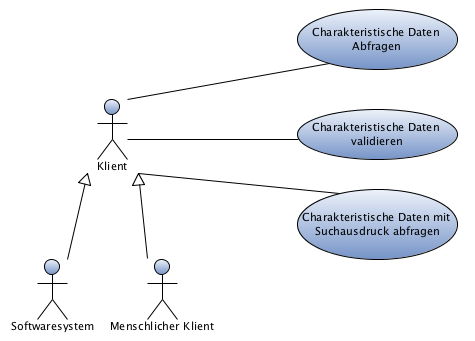
\includegraphics[width=0.75\textwidth]{images/usecases_plib.png}
	\caption{Use Case Übersicht}
	\label{fig:usecaseuebersicht}
\end{figure}

\subsection{Akteure}
Bei der Implementierung geht es um eine generische Schnittstelle. In den nachfolgenden Anwendungsfällen wird vom Akteur \enquote{Klient} gesprochen. Der Klient ist allgemein ein Nutzer der Schnittstelle, sei es als menschlicher Akteur welcher über eine Bedienerinterface die Schnittstelle benutzt oder eine direkte Maschinennutzung.    

%TODO Use Case Diagram

\subsection{Use Case Beschreibungen}

\subsubsection{Alle Charakteristische Daten eines Produkts abfragen}

{\small

\begin{description}
     \item[use case] Charakteristische Daten abfragen
     \item[  actors]~\\
     Klient
     \item[  precondition]~\\
     Der Klient verwendet einen gültigen Identifier.
     \item[  main flow]~\\
     Der Klient gibt einen Identifier (IRDI\footnote{International Registration Data Identifier}) einer Klasse von Elementen ein und sendet eine Anfrage ab. Die Anfrage wird auf Gültigkeit überprüft. Als Antwort bekommt er ein oder mehrere Datensätze von Elementen \footnote{Item, ISO 29002-10 Kapitel 5.3.2} mit den entsprechenden charakteristischen Daten \footnote{property\_values, ISO 29002-10 Kapitel 5.2.4}  des Elementes mit dem übergebenen Identifier zurück.
     \item[  postcondition]~\\
     Alle Daten aller Elemente der gewählten Klassen des Identifiers wurden zurückgegeben.    
     \item[  alternative flow] Properties auswählen ~\\
     Zusammen mit dem Identifier übergibt der Klient einen oder mehrere Property-Identifier und sendet diese erweiterte Anfrage ab.    
     \item[  postcondition]~\\
     Die mittels Property-Identifier ausgewählten Daten aller Elemente der gewählten Klassen wurden zurückgegeben.    
     \item[end] Charakteristische Daten abfragen
\end{description}

~\\

} %end small

\paragraph{Beispiel}

Ein Schraubendreher könnte folgendermaßen in einer Produktdatenbank repräsentiert werden:

\begin{description}\label{lab:schraubendreher}
\item[Klassen-Identifier] 0173-1\#01-AAA352\#4 
\item[Länge] 300mm
\item[Typ] Kreuz
\item[Spannungsfest] ja
\end{description}

Korrekterweise müssten anstatt der Attribute wie Länge oder Typ ebenfalls ein Identifier stehen. Die Benamungen sind hier zur besseren Lesbarkeit aufgelöst. 

Um nun alle Eigenschaften (Properties), wie Länge, Typ und Spannungsfest zu erhalten muss folgende Abfrage gesendet werden: 
\textbf{"Gib mir alle Items und alle Properties der Klasse mit dem Identifier 0173-1\#01-AAA352\#4 (Schraubendreher)".}
Das Ergebnis ist ein Item mit allen Attributen (Properties) der gewünschten Klassen und gegebenenfalls vorhandenen Unterklassen. In unserem Falle genau die oben angegebenen Werte.

Die XML-Abfrage sieht wie folgt aus:

\begin{lstlisting}[caption=Query Beispiel - Daten abfragen, language=XML, label=UseCaseDatenabfragen]
<?xml version="1.0" encoding="UTF-8"?>
<qy:query xsi:schemaLocation="...query query.xsd" xmlns:xsi="http://www.w3.org/2001/XMLSchema-instance" xmlns:cat="...catalogue" xmlns:val="...value" xmlns:qy="...query" xmlns:bas="...basic">
	<qy:class_ref>0173-1#01-AAA352#4</qy:class_ref>
</qy:query>
\end{lstlisting}

Eine Abfrage, welche die Properties der Klasse auswählt die zurückgeliefert werden sollen könnte lauten: 
\textbf{"Gib mir alle Items und die Properties Länge und Typ der Klasse mit dem Identifier 0173-1\#01-AAA352\#4 (Schraubendreher)".}
Das Ergebnis ist ein Item mit den gewünschten Attributen (Properties). 

Die XML-Abfrage:
\begin{lstlisting}[caption=Query Beispiel - Daten abfragen mit Propertyeinschränkung, language=XML, label=lst:UseCaseDatenabfragenProperty]

<?xml version="1.0" encoding="UTF-8"?>
<qy:query xsi:schemaLocation="...query query.xsd" xmlns:xsi="http://www.w3.org/2001/XMLSchema-instance" xmlns:cat="...catalogue" xmlns:val="...value" xmlns:qy="...query" xmlns:bas="...basic">
	<qy:class_ref>0173-1#01-AAA352#4</qy:class_ref>
	
	<!-- typ und laenge -->
	<qy:property_ref>0173-1#01-BBB111#1 0173-1#01-BBB222#1</qy:property_ref> 
	
</qy:query>
\end{lstlisting}

Listing \ref{lst:UseCaseDatenabfragenProperty} beinhaltet ein XML-Attribut property\_ref. Das wird mit gewünschten Property Identifier gefüllt, welche mit Leerzeichen getrennt werden. 

\subsubsection{Charakteristische Daten eines Produkts validieren}

{\small

\begin{description}
     \item[use case] Charakteristische Daten validieren
     \item[  actors]~\\
     Klient
     \item[  precondition]~\\
     Der Klient verwendet einen gültigen Identifier sowie auf den Identifier passende Daten..
     \item[  main flow]~\\
     Der Klient gibt einen Identifier eines Elementes (Klasse) ein. Zusätzlich übermittelt er zu diesem bekanntem Element Eigenschaften dieser Instanz des Elements und sendet eine Anfrage ab. Die Anfrage wird auf Gültigkeit überprüft. Als Antwort bekommt er ein oder mehrere Datensätze von Elementen mit den entsprechenden charakteristischen Daten zurück, auf welche die übergebenen Eigenschaften am besten zutreffen. 
     \item[  postcondition]~\\
     Alle Daten aller Elemente der gewählten Klassen des Identifiers werden zurückgegeben. Dies ermöglicht dem Klienten eine Validierung der ihm bereits bekannten Daten über ein Element. 
     \item[end] Charakteristische Daten validieren
\end{description}

~\\

} %end small

\paragraph{Beispiel}

In diesem Anwendungsfall verfügen wir bereits über Elemente/Wertenpaare einer bestimmten Klasse, z.B. eben jenen Schraubendreher

\textbf{"Ich habe hier ein mir bekanntes Item mit bestimmten Eigenschaften (Properties), Länge=300mm. Gib mir alle Items und alle Properties der Klasse mit dem Identifier 0173-1\#01-AAA352\#4 (Kreuzschraube) welche die mitgelieferten Eigenschaften haben".}
Das Ergebnis sind Items mit allen Properties der angegebenen Klasse, welche über die übergebenen Eigenschaften (Properties) verfügen. In unserem Fall vervollständigen wir unsere Properties mit den weiteren Properties "Typ" und "Spannungsfest".

Die XML-Abfrage sieht so aus:

\begin{lstlisting}[caption=Query Beispiel - Daten abfragen, language=XML, label=UseCaseDatenabfragen]
<?xml version="1.0" encoding="UTF-8"?>
<qy:query xsi:schemaLocation="...query query.xsd" xmlns:xsi="http://www.w3.org/2001/XMLSchema-instance" xmlns:cat="...catalogue" xmlns:val="...value" xmlns:qy="...query" xmlns:bas="...basic">
	<cat:item class_ref="0173-1#01-AAA352#4..">
		<cat:property_value property_ref="0173-1#01-BBB111#1">
			<val:integer_value></val:integer_value>
		</cat:property_value>
	</cat:item>
</qy:query>
\end{lstlisting}

\subsubsection{Chrarakteristische Daten mittels Suchausdruck abfragen }

{\small

\begin{description}
     \item[use case] Charakteristische Daten mit Suchausdruck abfragen
     \item[  actors]~\\
     Klient
     \item[  precondition]~\\
     Der Klient verwendet einen gültigen Identifier.
     \item[  main flow]~\\
     Der Klient gibt einen Identifier eines Elementes (Klasse) ein. Ferner übergibt er ein oder mehrere bekannte Property Identifier sowie passend dazu Werte zur Sucheinschränkung. 
     \item[  postcondition]~\\
     Alle Elemente auf jene diese Einschränkung der übergebenen Werte zutrifft wurden zurückgegeben. 
     \item[end] Charakteristische Daten mit Suchausdruck abfragen
\end{description}

~\\

} %end small

\paragraph{Beispiel}

Wir nehmen das Schraubendreher Beispiel aus \ref{lab:schraubendreher} zur Hand, und möchten eine Abfrage absenden, welche von der Klasse Schraubendreher alle Items erhalten soll die eine Länge zwischen 200 und 300 mm haben. 

Um nun alle Eigenschaften (Properties), wie Länge, Typ und Spannungsfest zu erhalten muss folgende Abfrage gesendet werden: 
\textbf{"Gib mir alle Items und alle Properties der Klasse mit dem Identifier 0173-1\#01-AAA352\#4 (Kreuzschraube)".}
Das Ergebnis ist ein Item mit allen Attributen (Properties) der gewünschten Klassen und gegebenenfalls vorhandenen Unterklassen. In unserem Falle genau die oben angegebenen Werte.

Die XML-Abfrage sieht so aus:

\begin{lstlisting}[caption=Query Beispiel - Daten abfragen, language=XML, label=UseCaseDatenabfragen]
<?xml version="1.0" encoding="UTF-8"?>
<qy:query xsi:schemaLocation="...query query.xsd" xmlns:xsi="http://www.w3.org/2001/XMLSchema-instance" xmlns:cat="...catalogue" xmlns:val="...value" xmlns:qy="...query" xmlns:bas="...basic">
	<qy:class_ref>0173-1#01-AAA352#4</qy:class_ref>
	<qy:characteristic_data_query_expression>
		<qy:range>
			<qy:property_reference property_ref="0173-1#01-BBB111#1"/>
			<qy:min_value>200</qy:min_value>
			<qy:max_value>300</qy:max_value>
			<qy:is_inclusive>true</qy:is_inclusive>
		</qy:range>
	</qy:characteristic_data_query_expression>
</qy:query>
\end{lstlisting}


%\section{Automatisierte Benutzerebene}
%Der Unterschied zur manuellen Benutzerebene ist der, dass hierbei automatisiert Daten angefragt und übermittelt werden. Es findet keine Mensch zu %Maschine Kommunikation statt sondern eine Maschine zu Maschine Kommunikation. 
%Ziel der automatisierten Anfragen ist das Abgleichen oder Validieren von Massendaten eines (Teil)-Katalogs. 

%\begin{description}
%\item[Alle Klassen abfragen] Der Klient sendet eine Anfrage und erhält alle vorhandene Klassen (ohne Items).
%\item[Items einer Klasse abgleichen] Der Klient möchte seine Daten abgleichen und fragt alle Items einer Klasse ab.  
%\item[Items einer Klasse validieren] Der Klient möchte seine Daten validieren und fragt alle Items einer Klasse ab.
%\end{description}
